\chapter{Results}

\section{Model Training Results}

In this section we will show progress and results of training the EfficientPose network on the three datasets presented in the previous chapter: the fully rendered dataset representing an M6x30 screw, henceforth referenced as "ScrewDataset", the augmented reality dataset representing a set of screws, henceforth "ScrewPose", and the augmented reality dataset representing the set of buttons and boards, henceforth "ButtonPose".

We will then be comparing these results with those obtained by EfficientPose on other datasets, namely LINEMOD for single object estimation and Occlusion-LINEMOD for multi-object estimation.

\begin{figure}[htp]
    \subfloat[Evolution using ScrewDataset for training.]{
        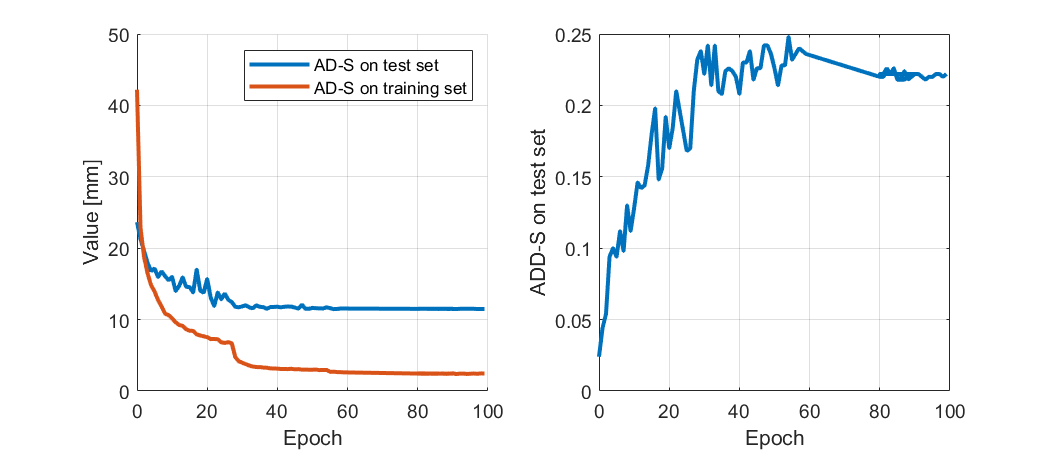
\includegraphics[width=0.8\textwidth]{screwdataset_training.png}
    }

    \subfloat[Evolution using ScrewPose for training.]{
        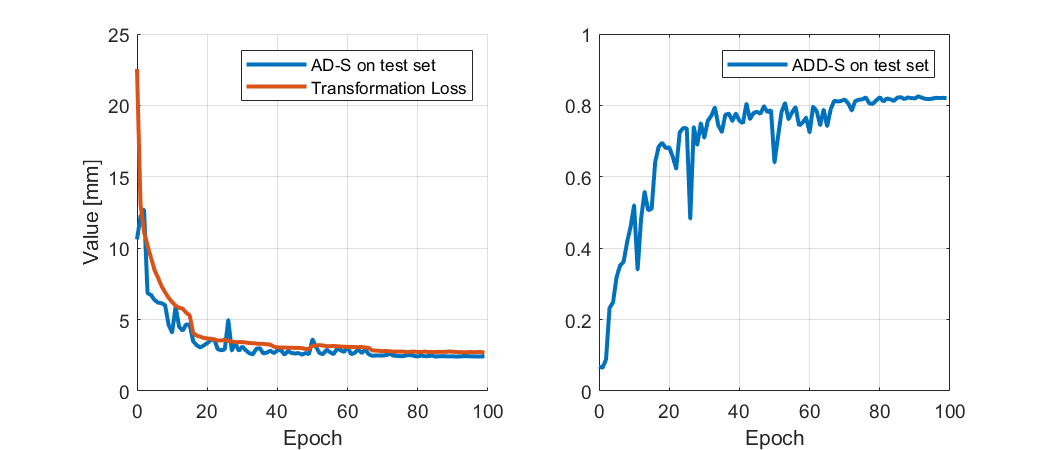
\includegraphics[width=0.8\textwidth]{screwpose_training.png}
    }

    \subfloat[Evolution using ButtonPose for training.]{
        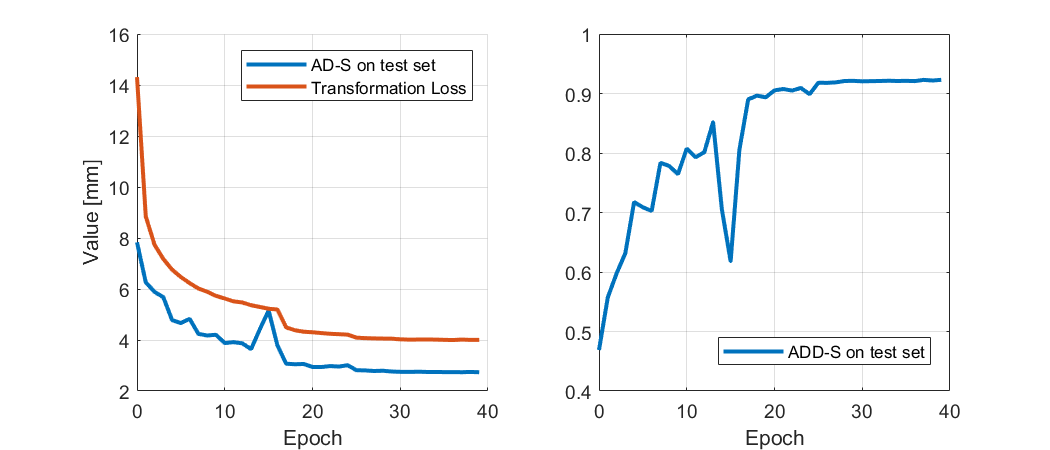
\includegraphics[width=0.8\textwidth]{buttonpose_training.png}
    }

    \caption{Training progress for EfficientPose on the ScrewDatset, ScrewPose and ButtonPose datsets, represented as the evolution of the transformation loss, AD-S and ADD-S metrics in evaluation for each epoch. Transformation loss is computed as the AD-S metric on the training dataset.}
\end{figure}

\begin{figure}[htp]
    \subfloat[ScrewDataset.]{
        \begin{tabular}{|c||c|c|c|}
            \hline
            Object & AP & AD-S [mm] & ADD-S \\
            \hline \hline
            M6x30 & 0.9675 & 11.4921 & 22.20\% \\
            \hline
        \end{tabular}
    }

    \subfloat[ScrewPose.]{
        \begin{tabular}{|c||c|c|c|}
            \hline
            Object & AP & AD-S [mm] & ADD-S \\
            \hline \hline
            M6x30 & 0.9399 & 2.1434 & 82.30\% \\
            M8x16 & 0.9538 & 1.9988 & 67.54\% \\
            M8x25 & 0.9645 & 2.1179 & 85.07\% \\
            M8x50 & 0.9880 & 3.4482 & 93.30\% \\
            \hline \hline
            Average & 0.9615 & 2.4271 & 82.05\% \\
            \hline    
        \end{tabular}
    }
    
    \subfloat[ButtonPose.]{
        \begin{tabular}{|c||c|c|c|}
            \hline
            Object & AP & AD-S [mm] & ADD-S \\
            \hline \hline
            2-slot & 0.9990 & 3.5420 & 99.90\% \\
            3-slot & 0.9985 & 3.9304 & 99.85\% \\
            red button & 0.9260 & 1.9825 & 86.01\% \\
            arrow button & 0.9349 & 2.0497 & 86.05\% \\
            safety button & 0.9962 & 2.6053 & 98.01\% \\
            unknown button & 0.9561 & 2.4757 & 82.95\% \\
            \hline \hline
            Average & 0.9685 & 2.76 & 92.13\% \\
            \hline    
        \end{tabular}
    }

    \caption{Evaluation of the Average Precision, Average Symmetric Distance, and ADD-S metrics on the ScrewDataset, ScrewPose and ButtonPose datasets after training.}
\end{figure}


On ScrewDataset, after 100 epochs of training the model has a final ADD of 22.20\%, with a peak value obtained during training of 24.8\%, much lower than the 97.35\% with $\phi=0$ reported by EfficientPose on LINEMOD. We can hypothesize that the reason for this performance gap is that the rendered dataset is much more difficult than LINEMOD, since we are dealing with a very small, symmetric object hidden inside a chaotic, colorful background with widely differing light conditions.

Another serious issue with this dataset, that is more difficult to convey on paper, is that the model is not able to bridge the reality gap: while testing in real-life scenarios, it failed to identify the screw in most conditions, let alone produce accurate estimations. This means that it generalises poorly outside of the simulated environment, making it essentially unuseable in real world applications.

On the flip side, the ScrewPose datset obtainined an average ADD-S of 82.05\%, which is better than EfficientPose's 79.04\% with $\phi=0$ on Occlusion-LINEMOD, and comparable to its 83.98\% with $\phi = 3$. This is a good result considering that the objects for our dataset are smaller, symmetric and all visually similar. Even though the Occlusion dataset is notoriously challenging, this anyways demonstrates the good performance of our own dataset. The model is also able to generalise to real life scenarios without noticeable losses in performance, as shown in figure \ref*{fig:inferencing}.

Finally, training on the ButtonPose dataset resulted in abnormally good performance for the boards, reaching over 99\% ADD-S and AP for both. The larger safety button also obtained great results, with a 98\% ADD-S, while the other buttons achieved more middling performances, but still better than the Occlusion-LINEMOD benchmark, showing that our approach is valid for more object sets. Noticeably, from this result and and the previous one it seems that performance for each object is proportional to its size: in both cases the network struggles with smaller objects (M8x16 screw, the smaller buttons), but performs much better with the larger ones (M8x50, the boards and larger safety button).

\begin{figure}[htp]
    \subfloat[ScrewPose.]{
        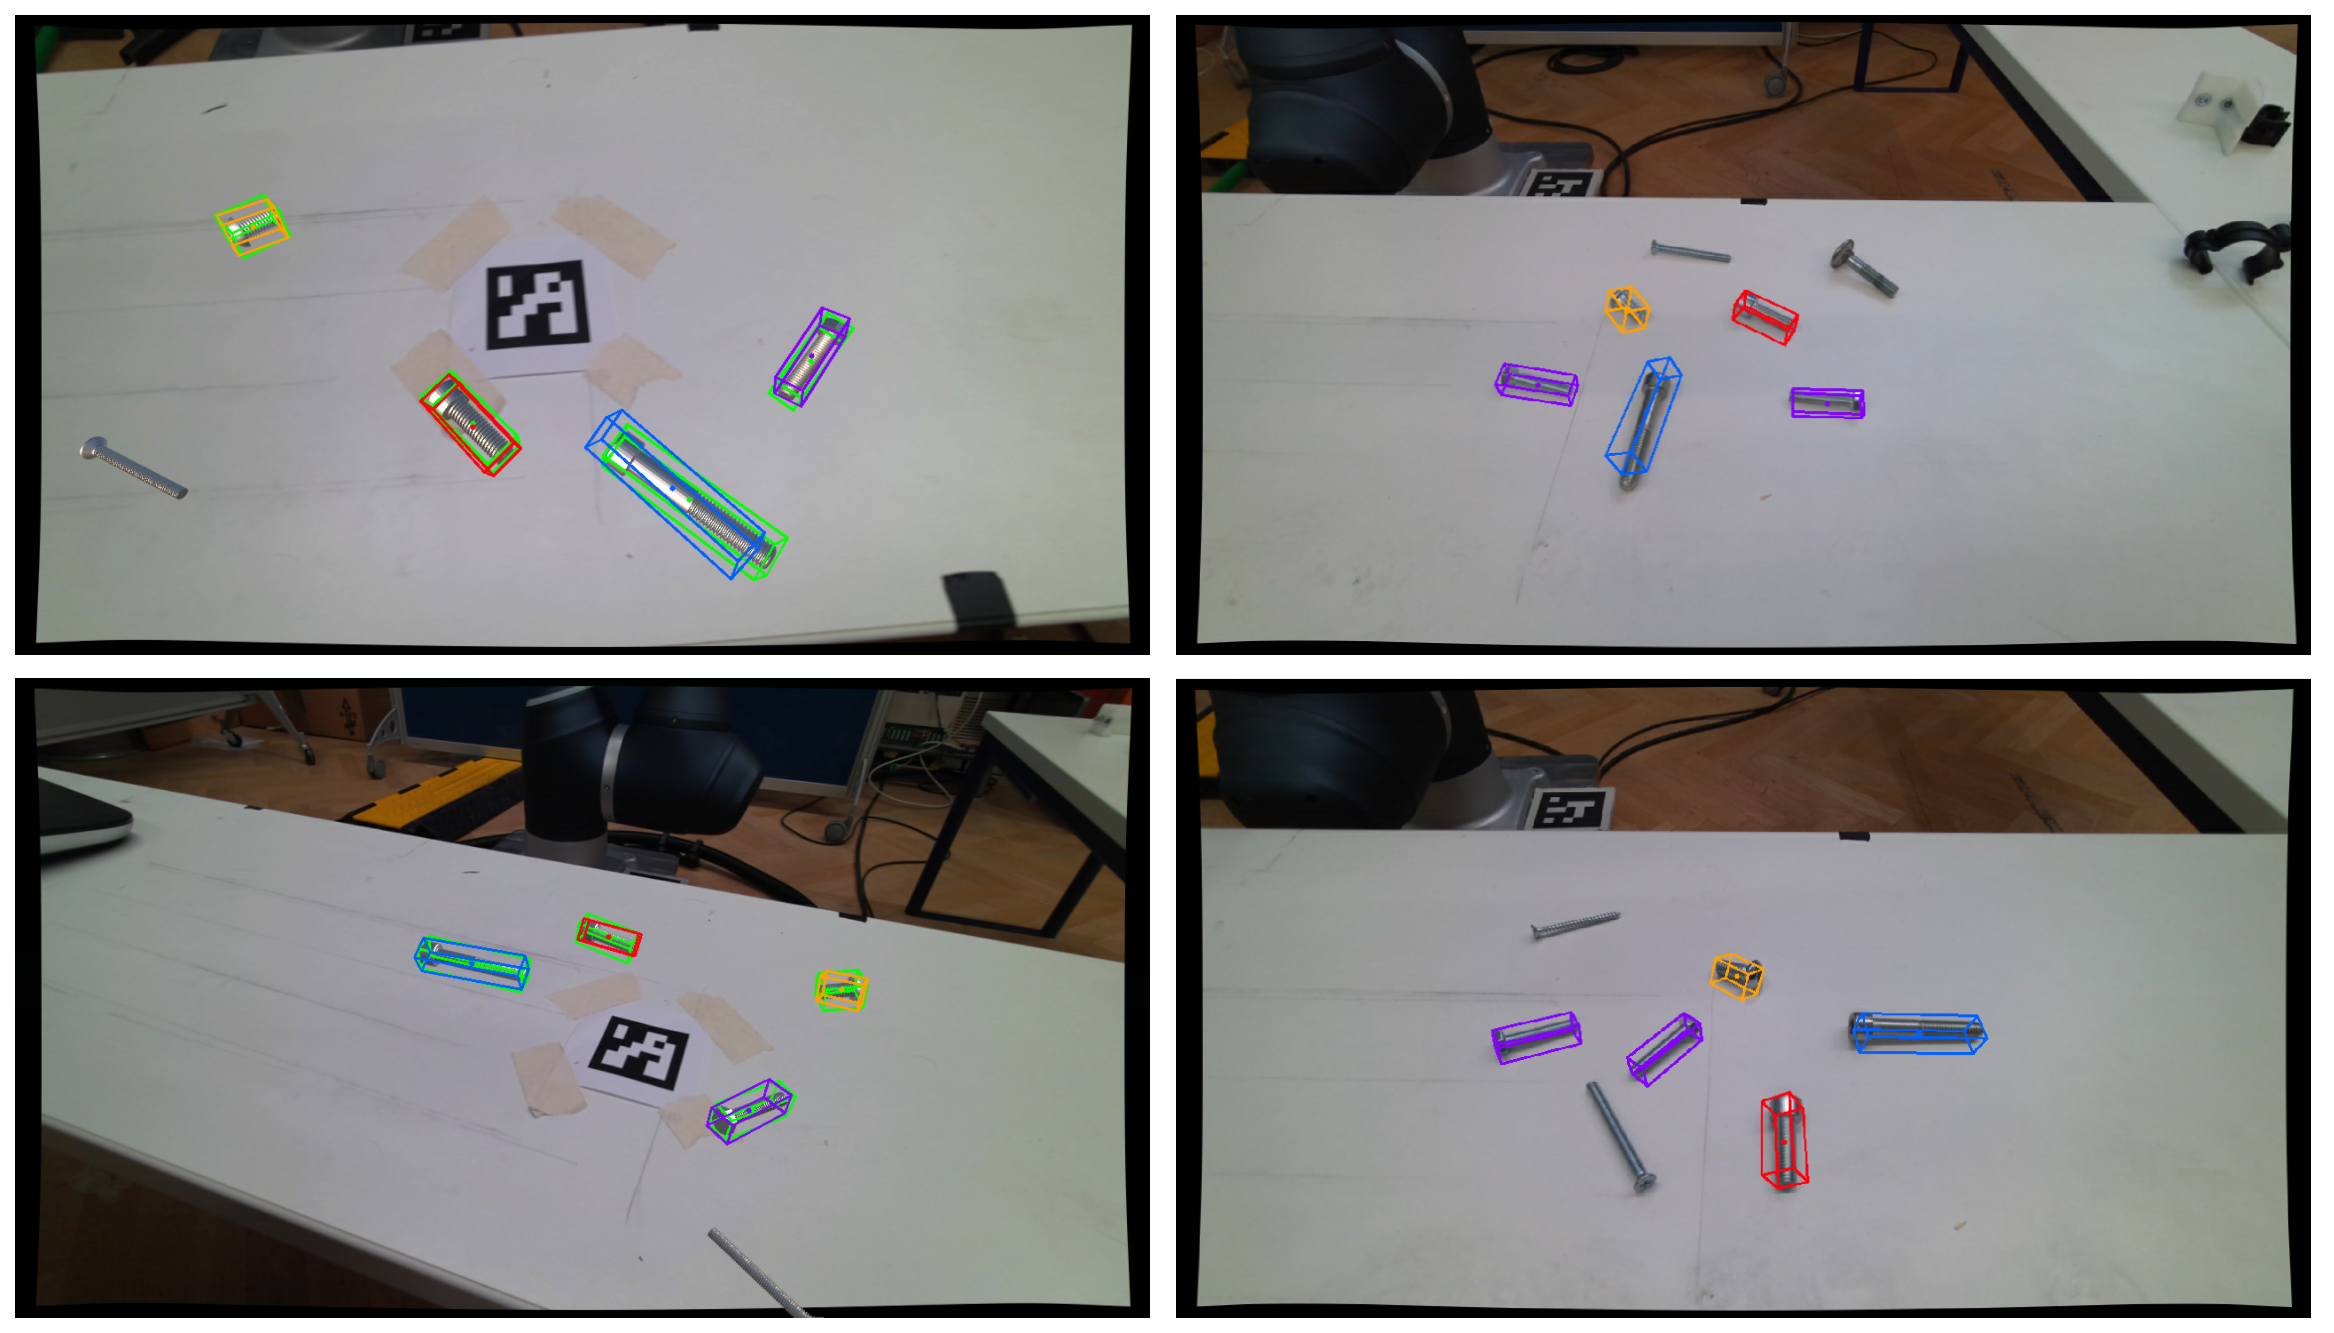
\includegraphics[width=\textwidth]{screwpose_inferencing.png}
    }

    \subfloat[ButtonPose.]{
        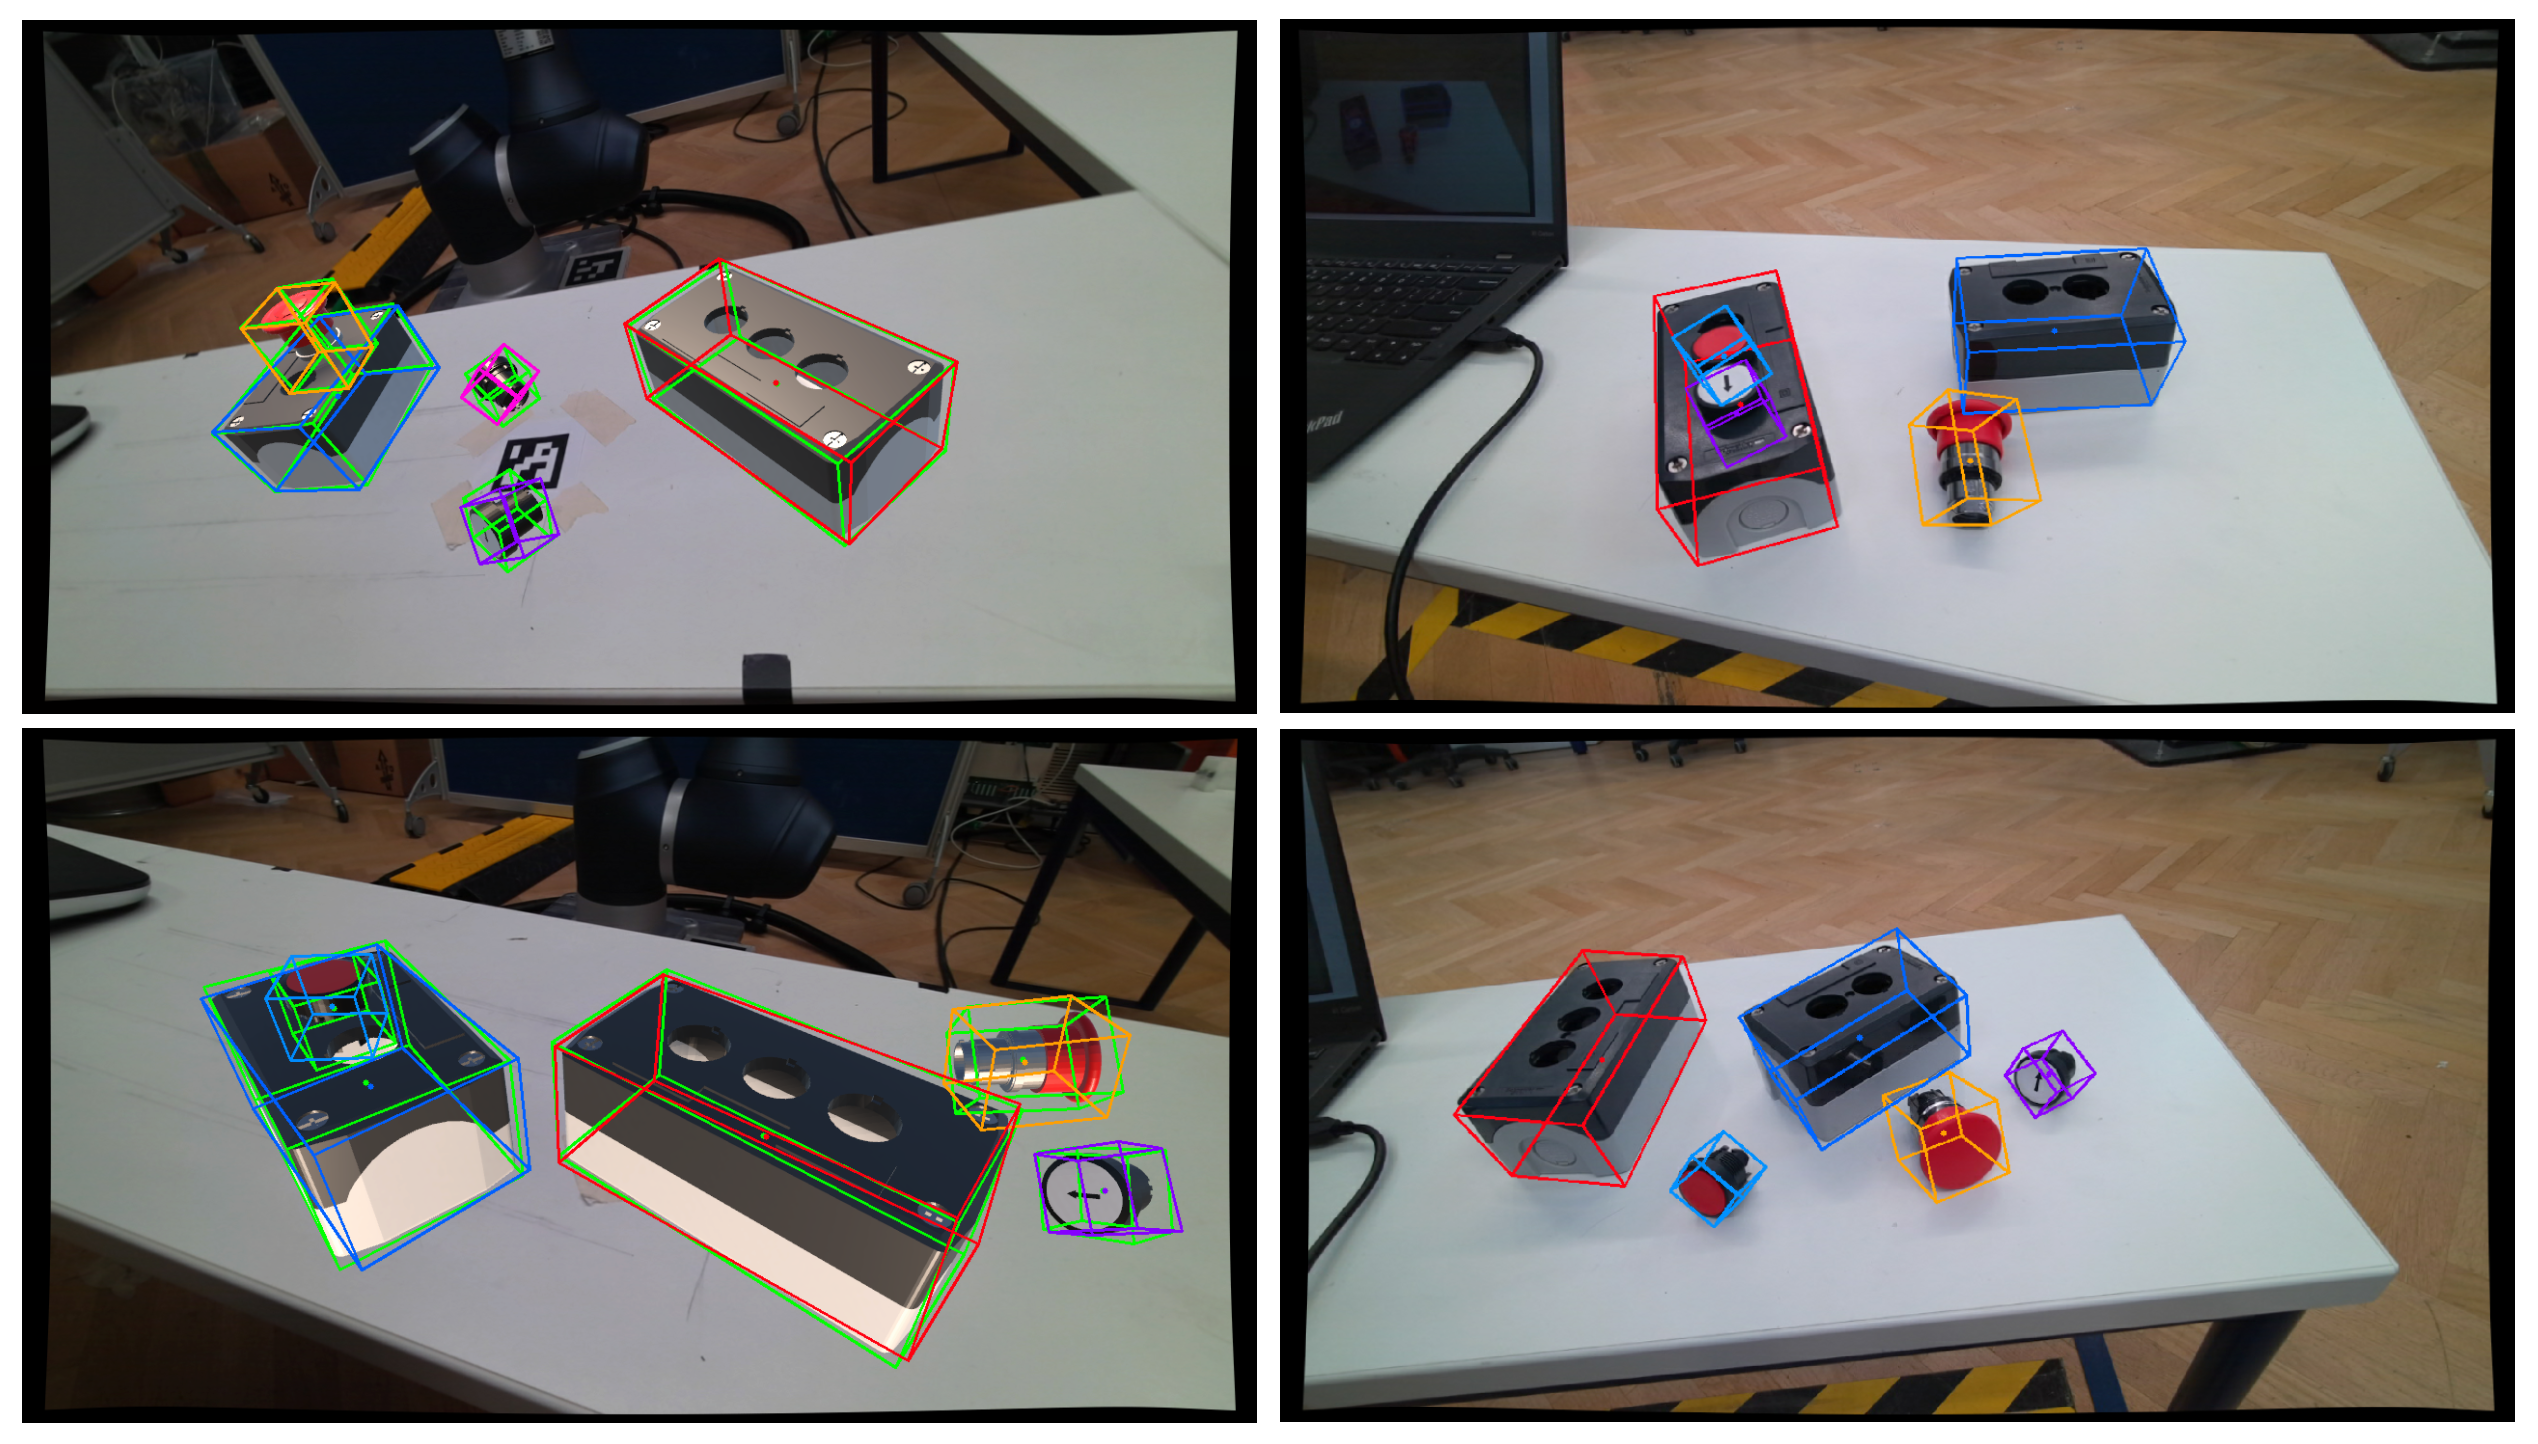
\includegraphics[width=\textwidth]{buttonpose_inferencing.png}
    }

    \caption{Images displaying pose estimations from the network for the ScrewPose and ButtonPose datasets. The left images are part of evaluation and display ground truths with green bounding boxes, the right ones are captures from a real camera in the testing environment.}
    \label{fig:inferencing}
\end{figure}

\Section{Impact of object dimensions and distance}

One noticeable result we observed after training was the impact that physical dimensions have on the final performance of the model for each object. Namely, larger and closer objects have much better performance than smaller and further objects. This is immediately noticeable in the ScrewPose dataset, where the larger M8x50 screw obtained the best results and the M8x16 obtained the worst.

To show how extreme these differences can be, we trained two additional models using new datasets based on the ButtonPose dataset. These two differ solely based on the background images: for the first one the backgrounds were captured from an approximate distance of 50 cm, while for the second one the backgrounds were captured from a distance of approximately 30 cm. For each of these conditions, we captured 50 backgrounds from a variety of positions at the same approximate distance from the marker. Our method for AR dataset generation proved to be a large asset in this, as creating these datasets was as simple as substituting the new backgrounds in the pipeline.

\Section{Semantic Meaning Extraction Results}

Given a binary classification problem such as ours (a button can either be in a slot or not), based on the output of our method we can build a confusion matrix as shown in table \ref{tab:cmatrix}.

\begin{table}[ht]
    \begin{center}
        \begin{tabular}{c||c|c}
            \space & Actual Positives & Actual Negatives\\
            \hline\hline
            Predicted Positives & True Positives (TP)& False Positives (FP)\\
            \hline
            Predicted Negatives & False Negatives (FN)& True Negatives (TN)\\
        \end{tabular}
        \caption{Generation of the confusion matrix.}
        \label{tab:cmatrix}
    \end{center}
\end{table}

We then define the precision and recall metrics as:

\begin{align*}
    \text{Precision} =& \frac{\text{TP}}{\text{TP}+\text{TN}} \\
    & \\
    \text{Recall} =& \frac{\text{TP}}{\text{TP}+\text{FN}}
\end{align*}

We want to maximise both of these metrics. To do this, we can plot them as a function of the threshold, and as a function of each other in a precision-recall graph, depicted in figure \ref{fig:precisionrecall}.

\begin{figure}[ht]
    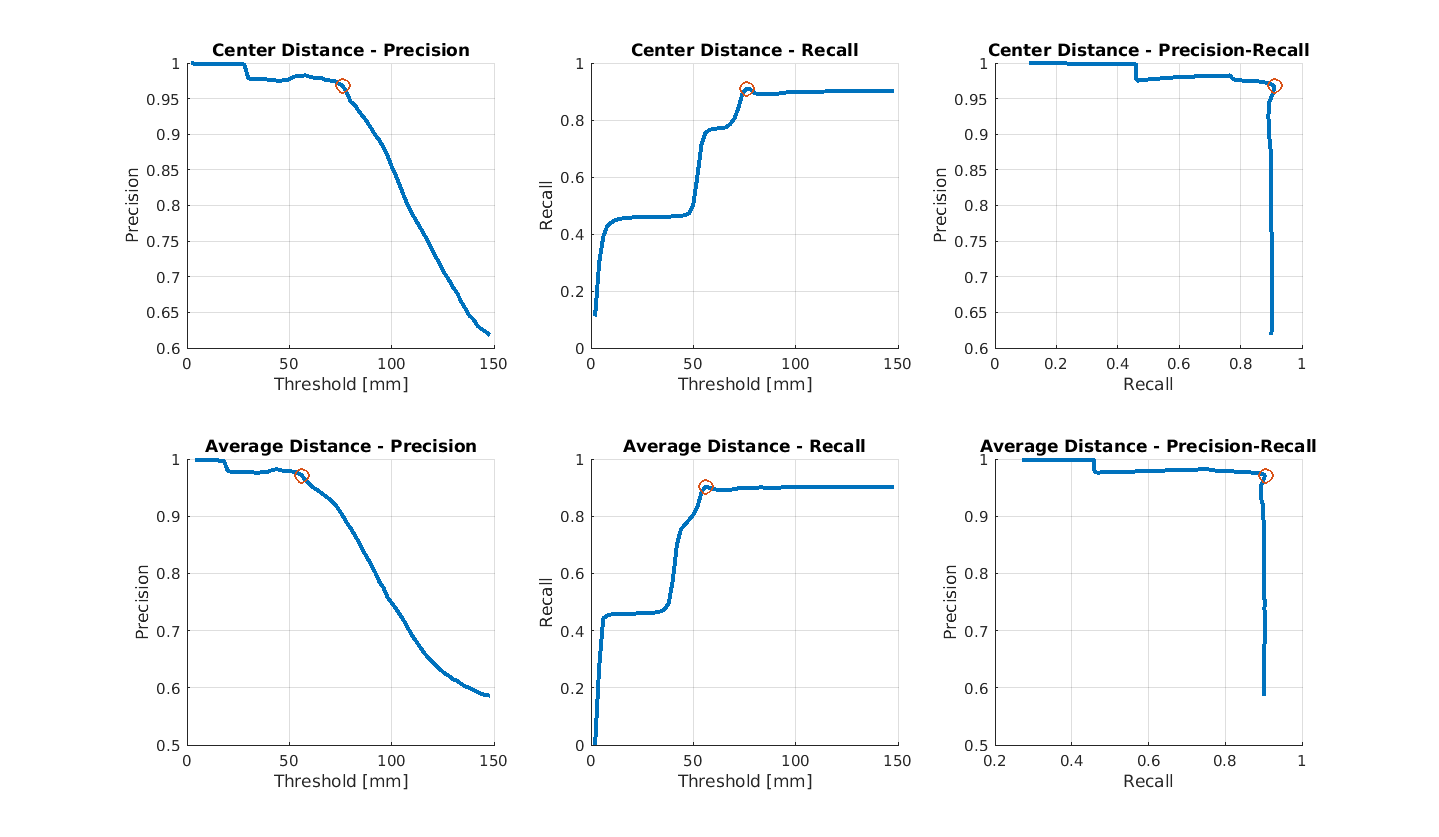
\includegraphics[width=\textwidth]{precision-recall.png}
    \caption{Precision and recall for both distance metrics on the Buttonpose dataset. The point with the best F1 score is highlighted with a red circle.}
    \label{fig:precisionrecall}
\end{figure}

As can be seen from the figure, higher thresholds greatly impact the precision of our model while lower thresholds greatly impact its recall. Overall we maintain high values, but our maximum recall is limited by the performance of the network to about 90\% for both distance metrics. To select the optimal threshold, we consider the F1 score, which is a balanced function of precision and recall:

\begin{equation*}
    \text{F1} = 2\times\frac{\text{Precision}\times\text{Recall}}{\text{Precision}+\text{Recall}}
\end{equation*}

For the average symmetric distance method, this results in a maximum F1 score of 0.9369, corresponding to a threshold of 56 mm, while for the center-to-center method the maximum is 0.9255, corresponging to a 78 mm threshold.

For our application we observe that there is no great advantage in using average distance over center-to-center. Given the additional complexity and computation time, the increase in performance is not significant.

We also obtained abnormally high thresholds for both methods. This can be attributed to the generated dataset: by stating that the buttons can only be either inside a slot or placed on the surface, we are in fact considering an ideal situation where a hypothetical manipulator does not commit any errors in picking up and inserting the buttons in their slots. If botched attempts are considered in the dataset, it is likely that the optimal threshold will be lower, and that the Average Distance method, being more sensible to situations with different rotations, may give better results than Center-to-Center.

Finally, the threshold is also influenced by the probability distribution we used for generating the poses for the button dataset, which in our case being a uniform distribution, resulted in a more spread-out placement, thus a higher optimal threshold. This is further compounded by the brute-force collision avoidance strategy implemented within the placement algorithm: if a placement attempt would generate an intersection with an already placed object, the placement was simply re-attempted from scratch. This naturally results in less conditions where dataset objects are in close proximity, and therefore in a higher threshold.


